\chapter{अनुकूली प्रतिरक्षा और टीकाकरण}\label{ch:b3:adaptive-immunity}

1796 में किसी देहाती डॉक्टर ने एक ग्वालिन के गोशीतला-फोड़े से पूय
खुरचकर किसी लड़के की बाँह में डाला, और छह सप्ताह बाद उसे चेचक का \omterm{def:b3:adaptive-immunity:vaccine}{टीका}
लगाया; लड़का बीमार नहीं पड़ा। 1980 में विश्व स्वास्थ्य संगठन ने उसी
विधि से चेचक को --- जिसने बीसवीं सदी में तीस करोड़ लोग मारे थे ---
पृथ्वी से उन्मूलित घोषित कर दिया। जिस तंत्र को जेनर ने, उसके होने की
जानकारी के बिना ही, काम पर लगा दिया था, वह किसी भी ऐसे अणु को पहचान
सकता है जिससे वह कभी न मिला हो, एक खरब भिन्न ग्राहियों में से उन थोड़ों
को चुन सकता है जो उस पर बैठते हैं, उन्हें ढोती कोशिकाएँ एक सप्ताह में
दस लाख गुना कर सकता है, ऐसा करते-करते उत्परिवर्तन और वरण से उनका बैठना
सुधार सकता है, और परिणाम जीवन भर याद रख सकता है; वह यह भी सीखता है कि
जिस शरीर ने उसे बनाया उस पर वार न करे, और यह सीखने की उसकी विफलताएँ ही
स्वप्रतिरक्षी रोग हैं। यह अध्याय \omterm{def:b3:adaptive-immunity:lymphocytes}{लसीकाणुओं} की बात करता है और यह कि वे
अपने ग्राही कैसे बनाते हैं, कोई अनुक्रिया कैसे खड़ी होती और याद रखी जाती
है, \omterm{def:b3:adaptive-immunity:tolerance}{सह्यता} कैसे लागू होती और कैसे टूटती है, और वह अंकगणित जिससे
पर्याप्त लोगों का टीकाकरण उन लोगों की भी रक्षा कर देता है जिनका नहीं
हुआ।

\section{लसीकाणु और क्लोनी वरण}

\begin{definition}[लसीकाणु और उनके ग्राही]\label{def:b3:adaptive-immunity:lymphocytes}
\index{लसीकाणु}\index{B कोशिका}\index{T कोशिका}\index{प्रतिजन}\index{क्लोनी वरण}\index{लसीका ग्रंथि}
\emph{अनुकूली प्रतिरक्षा} \emph{लसीकाणु} ढोते हैं: \emph{B कोशिकाएँ},
जो अस्थि-मज्जा में परिपक्व होती हैं और जिनका प्रतिजन-ग्राही कोई
झिल्ली-बद्ध \emph{\omterm{def:b3:adaptive-immunity:antibody}{प्रतिरक्षी}} है, जिसे वे बाद में स्रवित करती हैं; और
\emph{T कोशिकाएँ}, जो \omterm{def:b3:adaptive-immunity:tolerance}{थाइमस} में परिपक्व होती हैं और जिनका ग्राही दूसरी
कोशिकाओं के पृष्ठ पर दिखाए गए पेप्टाइड टुकड़े पहचानता है। कोई
\emph{प्रतिजन} वह है जो भी कोई ग्राही बाँधे; जो भाग सचमुच छुआ जाता है वह
कोई \emph{एपिटोप} है। नींव का तथ्य \emph{क्लोनी वरण} है (बर्नेट, 1957):
हर लसीकाणु केवल एक ही विशिष्टता के ग्राही ढोता है, जो किसी भी प्रतिजन
से मिलने से पहले तय हो चुके होते हैं; शरीर ऐसी कोई $10^{11}$ कोशिकाओं
का संग्रह रखता है; कोई प्रतिजन उन थोड़ी कोशिकाओं को चुन लेता है जिनके
ग्राही बैठते हैं और उन्हें कारक तथा \omterm{def:b3:adaptive-immunity:response}{स्मृति कोशिकाओं} के किसी क्लोन में
बँटने को प्रेरित करता है; और जिन लसीकाणुओं के ग्राही शरीर के अपने
अणुओं पर बैठते हैं वे परिपक्व होते समय ही मिटा या चुप कर दिए जाते हैं।
ये कोशिकाएँ रक्त और \emph{लसीका ग्रंथियों}, प्लीहा तथा श्लेष्मिक लसीकाभ
ऊतक के बीच लगातार घूमती रहती हैं, जहाँ \omterm{def:b3:innate-immunity:innate}{वृक्षाभ कोशिकाओं}
(\cref{ch:b3:innate-immunity}) से लाया गया प्रतिजन दिखाया जाता है,
ताकि वह दुर्लभ मेल खाती कोशिका --- किसी दिए एपिटोप के लिए एक लाख में
एक --- उसे दिन-दो दिन में पा ले।
\end{definition}

\begin{proof}[प्रमाण-सामग्री]
नॉसल और लेडरबर्ग (1958) ने प्रतिरक्षित चूहों के एकल \omterm{def:b3:adaptive-immunity:lymphocytes}{लसीकाणु} सूक्ष्म
बूँदों में रखे और हर एक के स्रवित \omterm{def:b3:adaptive-immunity:antibody}{प्रतिरक्षी} की जाँच की: हर कोशिका
दोनों \omterm{def:b3:adaptive-immunity:lymphocytes}{प्रतिजनों} में से किसी एक के विरुद्ध \omterm{def:b3:adaptive-immunity:antibody}{प्रतिरक्षी} बनाती थी, कभी
दोनों के विरुद्ध नहीं। बर्नेट ने इसका पूर्वानुमान एक वर्ष पहले कर दिया
था। टोनेगावा (1976) ने किसी प्रतिरक्षी-जीन का DNA भ्रूणीय कोशिकाओं में
और किसी प्रतिरक्षी-स्रावी \omterm{def:b3:cancer-biology:hallmarks}{अर्बुद} में मिलाकर देखा: भ्रूण में परिवर्ती
और अचर भाग दूर-दूर पड़े थे, \omterm{def:b3:cancer-biology:hallmarks}{अर्बुद} में वे जुड़े हुए --- वह जीन कायिक
कोशिका में काटा और जोड़ा गया था, यानी जान-बूझकर पुनर्विन्यस्त किए गए
किसी जीनोम का पहला प्रदर्शन।
\end{proof}

\section{एक खरब ग्राही बनाना}

\begin{definition}[प्रतिरक्षी की संरचना और V(D)J पुनर्संयोजन]\label{def:b3:adaptive-immunity:antibody}
\index{प्रतिरक्षी}\index{प्रतिरक्षी-ग्लोब्युलिन}\index{V(D)J पुनर्संयोजन}\index{RAG}\index{संधि-विविधता}\index{वर्ग-परिवर्तन}
कोई \emph{प्रतिरक्षी} (प्रतिरक्षी-ग्लोब्युलिन) दो एक जैसी भारी
शृंखलाएँ और दो एक जैसी हल्की शृंखलाएँ है, जिनमें से हर एक के सिरे पर
कोई \emph{परिवर्ती} प्रांत और पीछे \emph{अचर} प्रांत हैं; दोनों भुजाएँ
भारी प्रांत के तीन और हल्के परिवर्ती प्रांत के तीन अतिपरिवर्ती पाशों
से एक-एक एपिटोप बाँधती हैं, और डंठल (Fc) वही है जिसे भक्षककोशिकाएँ,
पूरक और मास्ट कोशिकाएँ पहचानती हैं। पाँच वर्ग अपने भारी-शृंखला अचर
क्षेत्र में भिन्न हैं: IgM, जो पहले बनता है, कोई पंचलक, जो पूरक अच्छी
तरह सक्रिय करता है; IgG, रक्त और ऊतकों का कर्मठ, जो अपरा पार करता है;
IgA, कोई द्विलक, जो श्लेष्मिक पृष्ठों के आर-पार आँत, वायुमार्गों और
दूध में स्रवित होता है; IgE, जो मास्ट कोशिकाओं से बँधा है, कृमियों के
विरुद्ध --- और एलर्जी का कारण; IgD। परिवर्ती प्रांत उसी रूप में
कूटबद्ध नहीं होते। भारी-शृंखला स्थल पर कोई $40$ प्रकार्यशील
\emph{V} खंड, $25$ \emph{D} और $6$ \emph{J} हैं; कोई विकसित होती
B~कोशिका हर एक में से एक चुनती है और उन्हें \emph{V(D)J पुनर्संयोजन}
से जोड़ देती है: एंज़ाइम RAG1 और RAG2 उन खंडों के किनारों पर पड़े
पुनर्संयोजन संकेत-अनुक्रमों पर काटती हैं, और सिरे
\cref{ch:b3:dna-repair} के असमजात सिरा-जोड़ तंत्र से जोड़ दिए जाते हैं,
और हर संधि पर न्यूक्लियोटाइड यादृच्छिक रूप से छाँटे और जोड़े जाते हैं
(एंज़ाइम TdT द्वारा) --- यही \emph{संधि-विविधता} है, जो ठीक तीसरे
अतिपरिवर्ती पाश में पड़ती है। हल्की शृंखलाएँ यही V और J के साथ करती
हैं। अनुक्रिया शुरू होने के बाद वही परिवर्ती प्रांत किसी दूसरे
पुनर्विन्यास से किसी भिन्न अचर क्षेत्र से जोड़ दिया जाता है, यानी
\emph{वर्ग-परिवर्तन}, जो प्रतिरक्षी का प्रकार्य बदल देता है, उसकी
विशिष्टता नहीं।
\end{definition}

\begin{theorem}[संग्रह का आकार]\label{thm:b3:adaptive-immunity:repertoire}
\index{संग्रह!संचयात्मक}
$V_{H} = 40$, $D = 25$, $J_{H} = 6$ भारी खंडों के साथ, और दो स्थलों से
आती हल्की शृंखलाओं के साथ जिनके $(V_{\kappa}, J_{\kappa}) = (40, 5)$
और $(V_{\lambda}, J_{\lambda}) = (30, 4)$ हों, केवल खंड-चयन से मिल
सकने वाले भिन्न भारी--हल्के संयोजनों की संख्या है
\[
(40\times 25\times 6)\times(40\times 5 + 30\times 4) = 6000\times 320
= 1.9\times 10^{6}.
\]
दो भारी संधियों और एक हल्की संधि पर \omterm{def:b3:adaptive-immunity:antibody}{संधि-विविधता} इसे $10^{4}$--$10^{5}$
की कोटि के किसी गुणक से गुणा कर देती है, जिससे $10^{10}$ से ऊपर का कोई
संभावित संग्रह बनता है, वह भी $200$ से कम जीन-खंडों से --- यानी किसी
शरीर की B~कोशिकाओं से भी अधिक, इसलिए असली संग्रह संभव संग्रह का कोई
प्रतिदर्श भर है। अनुक्रिया के दौरान \omterm{def:b3:adaptive-immunity:germinal-centre}{कायिक अतिउत्परिवर्तन} (नीचे) फिर हर
चुने गए ग्राही के प्रभेद बनाता है।
\end{theorem}
\begin{proof}
हर भारी शृंखला एक V, एक D और एक J है; हर हल्की शृंखला दोनों में से
किसी एक स्थल से एक V और एक J; कोई भी भारी किसी भी हल्की से जुड़ती है,
इसलिए गिनतियाँ गुणा होती हैं (गुणन नियम), और दोनों हल्के स्थल जुड़ते
हैं। संधि-गुणक उन भिन्न अनुक्रमों की संख्या है जो यादृच्छिक छँटाई और
जोड़ किसी संधि पर बना सकते हैं --- कम से कम कुछ दर्जन प्रति संधि ---
और उसे संधियों की संख्या के घात पर उठाया जाता है; उसका ठीक-ठीक मान
परिभाषित नहीं, पर तीन संधियाँ, हर एक $30$--$50$ परिणामों वाली,
$3\times 10^{4}$ से $10^{5}$ देती हैं। T~कोशिका ग्राहियों की गिनती,
जिनकी दो शृंखलाएँ उसी तरह पुनर्विन्यस्त होती हैं और जिनका संधि-योगदान
बड़ा है, उसी कोटि की है।
\end{proof}

\begin{omfigure}
\begin{tikzpicture}[every node/.style={font=\scriptsize}, >=stealth]
  % antibody Y
  \begin{scope}[xshift=0cm]
    % heavy chains
    \draw[very thick, omDef] (0,0) -- (0,1.6) -- (-1.3,3.0); \draw[very thick, omDef] (0.35,0) -- (0.35,1.6) -- (1.65,3.0);
    % light chains
    \draw[very thick, omProp] (-0.45,1.55) -- (-1.75,2.95); \draw[very thick, omProp] (0.8,1.55) -- (2.1,2.95);
    \fill[omThm] (-1.55,3.0) circle (0.12); \fill[omThm] (1.9,3.0) circle (0.12);
    \node[above, align=center] at (-1.5,3.15) {परिवर्ती प्रांत:\\प्रतिजन-बंधक स्थल}; 
    \node[right, align=left] at (0.55,0.5) {Fc डंठल (अचर):\\वर्ग प्रकार्य तय करता है};
    \node[left, omProp] at (-0.7,2.1) {हल्की}; \node[right, omDef] at (0.4,1.3) {भारी};
    \draw[omDef] (0.05,1.1) -- (0.3,1.1); \draw[omDef] (0.05,0.7) -- (0.3,0.7);
  \end{scope}
  % V(D)J locus
  \begin{scope}[xshift=4.2cm, yshift=2.4cm, xscale=0.86]
    \draw[very thick, gray] (0,0) -- (8.2,0);
    \foreach \x in {0.2,0.6,1.0,1.4} \draw[thick, fill=omDef!40] (\x,-0.15) rectangle (\x+0.3,0.15);
    \node[above] at (0.95,0.2) {V खंड ($\sim 40$)}; \node[font=\tiny] at (1.95,0) {$\cdots$};
    \foreach \x in {2.5,2.8,3.1} \draw[thick, fill=omProp!50] (\x,-0.15) rectangle (\x+0.2,0.15);
    \node[above] at (2.9,0.2) {D ($25$)};
    \foreach \x in {3.8,4.1,4.4} \draw[thick, fill=omMeth!50] (\x,-0.15) rectangle (\x+0.2,0.15);
    \node[above] at (4.2,0.2) {J ($6$)};
    \foreach \x/\lab in {5.3/\mu,6.0/\delta,6.7/\gamma,7.4/\alpha} { \draw[thick, fill=gray!30] (\x,-0.15) rectangle (\x+0.5,0.15); \node[above] at (\x+0.25,0.2) {C$_{\lab}$}; }
    \draw[->, thick] (4.1,-0.4) -- (4.1,-1.1) node[midway, right, align=left, font=\tiny] {RAG संकेत-अनुक्रमों पर काटती है; एक V, एक D,\\एक J जोड़े जाते हैं, TdT यादृच्छिक न्यूक्लियोटाइड जोड़ती है};
    % rearranged
    \draw[very thick, gray] (0,-1.5) -- (3.3,-1.5);
    \draw[thick, fill=omDef!40] (1.0,-1.65) rectangle (1.3,-1.35); \fill[omThm] (1.3,-1.65) rectangle (1.4,-1.35);
    \draw[thick, fill=omProp!50] (1.4,-1.65) rectangle (1.6,-1.35); \fill[omThm] (1.6,-1.65) rectangle (1.7,-1.35);
    \draw[thick, fill=omMeth!50] (1.7,-1.65) rectangle (1.9,-1.35);
    \draw[thick, fill=gray!30] (2.6,-1.65) rectangle (3.1,-1.35); \node[above] at (2.85,-1.3) {C$_{\mu}$};
    \node[below, align=center] at (1.45,-1.7) {VDJ जुड़ा: परिवर्ती प्रांत,\\लाल: संधि-न्यूक्लियोटाइड};
    \node[right, align=left, font=\tiny] at (3.4,-2.0) {C$_{\mu}$ से स्प्लाइस: कोई IgM भारी शृंखला;\\वर्ग-परिवर्तन बाद में उसी VDJ को\\C$_{\gamma}$ या C$_{\alpha}$ से जोड़ देता है};
  \end{scope}
\end{tikzpicture}

{\small बाएँ: कोई \omterm{def:b3:adaptive-immunity:antibody}{प्रतिरक्षी} --- दो भारी और दो हल्की शृंखलाएँ, सिरों पर
परिवर्ती प्रांत, जो दो बंधक स्थल बनाते हैं, और वह अचर डंठल जिसे बाकी
प्रतिरक्षा-तंत्र पढ़ता है। दाएँ: \omterm{def:b3:adaptive-immunity:antibody}{V(D)J पुनर्संयोजन} से पहले और बाद
भारी-शृंखला स्थल, जो हर तरह का एक-एक खंड उठाता है और जोड़ों पर
यादृच्छिक न्यूक्लियोटाइड जोड़ देता है।}
\end{omfigure}

\begin{definition}[T~कोशिका ग्राही और MHC]\label{def:b3:adaptive-immunity:mhc}
\index{T कोशिका ग्राही}\index{मुख्य ऊतक-संगतता संकुल}\index{प्रतिजन-प्रस्तुति}\index{MHC-प्रतिबंधन}\index{HLA}
\emph{T~कोशिका ग्राही} उसी पुनर्संयोजन से बना कोई दो-शृंखला अणु है, जो
कभी स्रवित नहीं होता, और वह विलयन में मुक्त पड़े \omterm{def:b3:adaptive-immunity:lymphocytes}{प्रतिजन} को नहीं
बाँधता: वह किसी दूसरी कोशिका के पृष्ठ पर बैठे \emph{मुख्य ऊतक-संगतता
संकुल} (MHC) अणु की खाँच में थमा कोई छोटा पेप्टाइड पहचानता है।
\emph{MHC वर्ग~I}, जो हर केंद्रकयुक्त कोशिका पर है, कोशिका के अपने
कोशिकाद्रव्यी प्रोटीनों से प्रोटिएसोम द्वारा काटे आठ से दस अवशेषों के
पेप्टाइड --- यानी कोशिका जो बना रही है उसका कोई प्रतिदर्श, किसी भी
\omterm{def:b3:virology:virus}{विषाणु} समेत --- \emph{CD8} T~कोशिकाओं को दिखाता है, जो पेप्टाइड पराया
हो तो उस कोशिका को मार देती हैं। \emph{MHC वर्ग~II}, जो \omterm{def:b3:innate-immunity:innate}{वृक्षाभ
कोशिकाओं}, \omterm{def:b3:innate-immunity:innate}{महाभक्षकों} और B~कोशिकाओं पर है, उन प्रोटीनों से आते तेरह से
पच्चीस अवशेषों के पेप्टाइड दिखाता है जिन्हें कोशिका ने भीतर लेकर
\omterm{def:b3:membrane-traffic:endocytosis}{अंतःकायों} में पचाया है, और वह उन्हें \emph{CD4} T~कोशिकाओं को दिखाता
है, जो मदद देकर अनुक्रिया करती हैं। कोई T~कोशिका \emph{प्रतिबंधित}
होती है: वह अपना पेप्टाइड केवल उसी MHC युग्मविकल्पी पर पहचानती है
जिस पर उसका वरण हुआ था। MHC जीन (मनुष्यों में \emph{HLA}) जीनोम में
सबसे बहुरूपी हैं, जिनके हज़ारों युग्मविकल्पी हैं और हर एक की खाँच अलग
है, ताकि हर व्यक्ति हर प्रोटीन के पेप्टाइडों का कोई भिन्न प्रतिदर्श
दिखाए और कोई रोगजनक सबमें प्रस्तुति से बच न सके --- और इसीलिए किसी
बेमेल दाता से प्रत्यारोपित अंग ग्रहीता की T~कोशिकाओं के बड़े अंश को
पराया दिखता है।
\end{definition}

\begin{proof}[प्रमाण-सामग्री]
ज़िंकरनागल और डोहर्टी (1974) ने दो अंतःप्रजनित प्रभेदों के चूहों को किसी
\omterm{def:b3:virology:virus}{विषाणु} से संक्रमित किया और उनकी कोशिकाविषी T~कोशिकाएँ संक्रमित
लक्ष्य-कोशिकाओं पर आज़माईं: T~कोशिकाओं ने अपने ही प्रभेद की संक्रमित
कोशिकाएँ मारीं, दूसरे प्रभेद की नहीं, जबकि \omterm{def:b3:virology:virus}{विषाणु} वही था। T~कोशिका ने
\omterm{def:b3:virology:virus}{विषाणु} को केवल किसी स्व MHC अणु के साथ ही देखा --- यानी
\emph{\omterm{def:b3:adaptive-immunity:mhc}{MHC-प्रतिबंधन}} --- जिसकी व्याख्या बाद में तब हुई जब किसी MHC अणु
की क्रिस्टल संरचना (ब्योर्कमैन, 1987) ने कोई ऐसी खाँच दिखाई जिसमें कोई
पेप्टाइड पड़ा था, और T~कोशिका ग्राही को दोनों को साथ बाँधते दिखाया गया।
\end{proof}

\begin{omfigure}
\begin{tikzpicture}[every node/.style={font=\scriptsize}, >=stealth]
  % class I pathway
  \begin{scope}
    \draw[thick, omDef, fill=omDef!8] (0,0) rectangle (6.2,3.6); \node[anchor=north west] at (0.05,3.55) {कोई भी केंद्रकयुक्त कोशिका};
    \node[draw, rounded corners, fill=omThm!20, font=\tiny, align=center] (v) at (1.4,2.6) {कोशिकाद्रव्य में विषाणुजन्य\\या स्व प्रोटीन};
    \node[draw, rounded corners, fill=gray!20, font=\tiny, align=center] (p) at (1.4,1.5) {प्रोटिएसोम:\\8--10 के पेप्टाइड};
    \node[draw, rounded corners, fill=omDef!25, font=\tiny, align=center] (er) at (4.6,1.5) {ER: MHC वर्ग I\\पर लदे};
    \draw[->, thick] (v) -- (p); \draw[->, thick] (p) -- node[midway, above, font=\tiny] {TAP} (er);
    \draw[->, thick] (er) -- (4.6,3.55);
    \draw[thick, fill=omDef!40] (4.4,3.6) rectangle (4.8,4.1); \fill[omThm] (4.6,4.2) circle (0.09);
    \node[above, align=center] at (4.6,4.35) {पेप्टाइड--MHC I\\CD8 T कोशिकाएँ देखती हैं: मारो};
  \end{scope}
  % class II pathway
  \begin{scope}[xshift=7.2cm]
    \draw[thick, omProp, fill=omProp!8] (0,0) rectangle (6.2,3.6); \node[anchor=north west] at (0.05,3.55) {वृक्षाभ कोशिका, महाभक्षक, B कोशिका};
    \node[draw, rounded corners, fill=omThm!20, font=\tiny, align=center] (ex) at (1.4,2.6) {किसी अंतःकाय में\\लिया गया प्रोटीन};
    \node[draw, rounded corners, fill=gray!20, font=\tiny, align=center] (dig) at (1.4,1.5) {पचा हुआ:\\13--25 के पेप्टाइड};
    \node[draw, rounded corners, fill=omProp!30, font=\tiny, align=center] (m2) at (4.6,1.5) {MHC वर्ग II\\यहीं लदा};
    \draw[->, thick] (ex) -- (dig); \draw[->, thick] (dig) -- (m2);
    \draw[->, thick] (m2) -- (4.6,3.55);
    \draw[thick, fill=omProp!50] (4.4,3.6) rectangle (4.8,4.1); \fill[omThm] (4.6,4.2) circle (0.09);
    \node[above, align=center] at (4.6,4.35) {पेप्टाइड--MHC II\\CD4 T कोशिकाएँ देखती हैं: मदद};
  \end{scope}
\end{tikzpicture}

{\small दोनों प्रस्तुति-पथ। वर्ग~I, CD8 T~कोशिकाओं को दिखाता है कि कोई
कोशिका अपने भीतर क्या बना रही है; वर्ग~II, CD4 T~कोशिकाओं को दिखाता है
कि किसी प्रतिजन-प्रस्तोता कोशिका ने क्या खाया है। कोशिकाविषी अनुक्रिया
पहले पर सधी है, सहायक अनुक्रिया दूसरे पर।}
\end{omfigure}

\section{अनुक्रिया}

\begin{definition}[सक्रियण, मदद और मारना]\label{def:b3:adaptive-immunity:response}
\index{सहायक T कोशिका}\index{कोशिकाविषी T कोशिका}\index{सह-उद्दीपन}\index{नियामक T कोशिका}\index{प्लाज़्मा कोशिका}\index{स्मृति कोशिका}
कोई अनुभवहीन T~कोशिका तब सक्रिय होती है जब उसका ग्राही किसी ऐसी \omterm{def:b3:innate-immunity:innate}{वृक्षाभ
कोशिका} पर पेप्टाइड--MHC बाँधे जो सह-उद्दीपन भी देती हो
(\cref{ch:b3:innate-immunity}); फिर वह एक सप्ताह तक हर छह से आठ घंटे
में बँटती और विभेदित होती है। \emph{CD4 सहायक} T~कोशिकाएँ, \omterm{def:b3:innate-immunity:innate}{वृक्षाभ
कोशिका} के \omterm{def:b3:innate-immunity:inflammation}{साइटोकाइनों} के अनुसार, उपसमुच्चयों में विभेदित होती हैं:
Th1, जो \omterm{def:b3:innate-immunity:innate}{महाभक्षकों} को वह मारने के लिए सक्रिय करती हैं जो उन्होंने खाया
है (तपेदिक); Th2, जो कृमियों के विरुद्ध IgE और इओसिनोफिल चलाती हैं;
Th17, जो बाह्यकोशिकीय जीवाणुओं तथा कवकों के विरुद्ध \omterm{def:b3:innate-immunity:innate}{न्यूट्रोफिल} बुलाती
हैं; पुटकीय सहायक, जो B~कोशिकाओं की मदद करती हैं; और \emph{नियामक}
T~कोशिकाएँ, जो दमन करती हैं। \emph{CD8 कोशिकाविषी} T~कोशिकाएँ उन
कोशिकाओं को मारती हैं जो अपना पेप्टाइड वर्ग~I पर दिखाएँ, परफ़ोरिन तथा
ग्रैन्ज़ाइमों से और Fas बंधक से, जिससे \omterm{def:b3:cell-cycle-apoptosis:apoptosis}{एपॉप्टोसिस} छिड़ जाता है
(\cref{ch:b3:cell-cycle-apoptosis}) --- यही \omterm{def:b3:virology:virus}{विषाणुओं} और \omterm{def:b3:cancer-biology:hallmarks}{अर्बुदों} के
विरुद्ध बचाव है। कोई B~कोशिका तब सक्रिय होती है जब \omterm{def:b3:adaptive-immunity:lymphocytes}{प्रतिजन} उसका ग्राही
बाँधे और साथ ही किसी पुटकीय सहायक T~कोशिका से मदद मिले, जो उसी \omterm{def:b3:adaptive-immunity:lymphocytes}{प्रतिजन}
के पेप्टाइड उस B~कोशिका के वर्ग~II पर पहचानती है; फिर वह कोई
\emph{प्लाज़्मा कोशिका} बन जाती है, जो प्रति सेकंड हज़ारों \omterm{def:b3:adaptive-immunity:antibody}{प्रतिरक्षी}
स्रवित करती है, कुछ दिनों तक (अल्पजीवी, ग्रंथि में) या वर्षों तक
(दीर्घजीवी, मज्जा में), या किसी \omterm{def:b3:adaptive-immunity:germinal-centre}{जनन-केंद्र} में चली जाती है।
\emph{स्मृति} B और T~कोशिकाएँ --- दीर्घजीवी, अनुभवहीन पूर्वजों से अधिक
संख्या में और अनुक्रिया में तेज़ --- हर अनुक्रिया की बचत हैं और
टीकाकरण का आधार।
\end{definition}

\begin{definition}[जनन-केंद्र]\label{def:b3:adaptive-immunity:germinal-centre}
\index{जनन-केंद्र}\index{कायिक अतिउत्परिवर्तन}\index{बंधुता-परिपक्वन}
किसी \emph{जनन-केंद्र} में, यानी उस संरचना में जो किसी अनुक्रिया के कोई
सप्ताह भर बाद किसी \omterm{def:b3:adaptive-immunity:lymphocytes}{लसीका ग्रंथि} में बनती है, सक्रिय B~कोशिकाएँ कोई
विकासीय कलन-विधि चलाती हैं। उसके गहरे क्षेत्र में वे हर छह घंटे में
बँटती हैं और उनके प्रतिरक्षी-परिवर्ती जीन एंज़ाइम AID द्वारा प्रति
विभाजन प्रति हज़ार क्षार-युग्म लगभग एक बदलाव की दर से उत्परिवर्तित किए
जाते हैं --- यही \emph{कायिक अतिउत्परिवर्तन} है, जो जीनोमी दर से दस
लाख गुना है और किसी एक किलोक्षार पर सधा हुआ। हलके क्षेत्र में हर
कोशिका अपना नया ग्राही उस \omterm{def:b3:adaptive-immunity:lymphocytes}{प्रतिजन} के सामने आज़माती है जो पुटकीय \omterm{def:b3:innate-immunity:innate}{वृक्षाभ
कोशिकाओं} पर थमा है, और T~कोशिकाओं की मदद के लिए स्पर्धा करती है: जो
कोशिकाएँ बेहतर बाँधती हैं वे अधिक \omterm{def:b3:adaptive-immunity:lymphocytes}{प्रतिजन} भीतर लेती हैं, अधिक
प्रस्तुत करती हैं, अधिक मदद पाती हैं और फिर बँटने के लिए गहरे क्षेत्र
में लौट जाती हैं; जो खराब बाँधती हैं, या बाँधना खो चुकी हैं, वे
\omterm{def:b3:cell-cycle-apoptosis:apoptosis}{एपॉप्टोसिस} से मर जाती हैं। दो से तीन सप्ताह के चक्रों में बचे
\omterm{def:b3:adaptive-immunity:antibody}{प्रतिरक्षियों} की बंधुता सौ से हज़ार गुना चढ़ जाती है --- यही
\emph{बंधुता-परिपक्वन} है --- और विजेता \omterm{def:b3:adaptive-immunity:response}{प्लाज़्मा कोशिकाओं} तथा \omterm{def:b3:adaptive-immunity:response}{स्मृति
कोशिकाओं} के रूप में निकलते हैं, अपना वर्ग भी बदलकर। द्वितीयक अनुक्रिया
इसलिए तेज़, बड़ी और बेहतर \omterm{def:b3:adaptive-immunity:antibody}{प्रतिरक्षी} की बनी होती है कि वह इसी चुनी हुई,
फैली हुई, वर्ग बदल चुकी समष्टि से शुरू होती है।
\end{definition}

\begin{omfigure}
\begin{tikzpicture}[every node/.style={font=\scriptsize}, >=stealth]
  \draw[thick, omDef, fill=omDef!12] (0,0) ellipse (2.7 and 1.7); \node[above, omDef!70!black] at (0,1.75) {गहरा क्षेत्र};
  \draw[thick, omMeth!70!black, fill=omMeth!12] (6.2,0) ellipse (2.7 and 1.7); \node[above, omMeth!60!black] at (6.2,1.75) {हलका क्षेत्र};
  \node[align=center] at (0,0.3) {B कोशिकाएँ हर \qty{6}{h} में बँटतीं;\\AID प्रतिरक्षी जीन उत्परिवर्तित करती है:\\प्रति bp प्रति विभाजन $10^{-3}$};
  \node[align=center] at (6.2,0.3) {नया ग्राही उस प्रतिजन पर\\आज़माएँ जो पुटकीय वृक्षाभ\\कोशिकाओं पर थमा है;\\T कोशिका की मदद के लिए स्पर्धा};
  \draw[->, very thick, omProp] (2.4,0.7) .. controls (3.6,1.4) and (4.2,1.4) .. (3.7,0.7); \node[above, omProp] at (3.1,1.45) {उत्परिवर्ती बाहर};
  \draw[->, very thick, omMeth!70!black] (3.7,-0.7) .. controls (4.2,-1.4) and (3.6,-1.4) .. (2.4,-0.7); \node[below, omMeth!70!black] at (3.1,-1.45) {विजेता वापस, फिर बँटने};
  \draw[->, thick, omThm] (6.6,-1.6) -- (6.6,-2.3); \node[below, omThm, align=center] at (6.6,-2.3) {हारे: एपॉप्टोसिस\\(अधिकांश)};
  \draw[->, thick] (8.9,0) -- (9.5,0); \node[right, align=left] at (9.5,0) {2--3 सप्ताह बाद:\\प्लाज़्मा कोशिकाएँ (दीर्घजीवी,\\मज्जा में) और स्मृति\\B कोशिकाएँ; बंधुता\\$100$--$1000\times$ ऊपर, वर्ग बदला};
\end{tikzpicture}

{\small किसी विकासीय यंत्र के रूप में \omterm{def:b3:adaptive-immunity:germinal-centre}{जनन-केंद्र}: गहरे क्षेत्र में
उत्परिवर्तन, हलके में वरण, और दोनों के बीच चक्र तब तक, जब तक निकलते
\omterm{def:b3:adaptive-immunity:antibody}{प्रतिरक्षी} घुसे हुओं से कहीं बेहतर न बाँधने लगें।}
\end{omfigure}

\begin{example}[किसी अनुक्रिया की बलगतिकी]\label{ex:b3:adaptive-immunity:kinetics}
$10^{5}$ में लगभग एक B~कोशिका कोई दिया एपिटोप बाँधती है, इसलिए किसी
शरीर की $10^{11}$ B~कोशिकाओं में कोई $10^{6}$ पूर्वज होते हैं, जिनमें
से शायद सौ निकास ग्रंथि में उस \omterm{def:b3:adaptive-immunity:lymphocytes}{प्रतिजन} से मिलते हैं। हर आठ घंटे में
बँटते हुए सौ कोशिकाएँ एक सप्ताह में
$10^{2}\times 2^{21} \approx 2\times 10^{8}$ हो जाती हैं। सीरम में \omterm{def:b3:adaptive-immunity:antibody}{प्रतिरक्षी} चार से छह दिन बाद
प्रकट होता है, पहले IgM, कोई दो सप्ताह में शिखर छूता है और IgG के लिए
तीन सप्ताह के अर्ध-आयु काल से घटता है, क्योंकि अल्पजीवी \omterm{def:b3:adaptive-immunity:response}{प्लाज़्मा
कोशिकाएँ} मर जाती हैं, और अंततः उस स्तर पर ठहरता है जिसे दीर्घजीवी
मज्जा-प्लाज़्मा कोशिकाएँ वर्षों बनाए रखती हैं। दूसरा संसर्ग ऊँची
बंधुता की, पहले ही IgG में बदल चुकी $10^{4}$--$10^{5}$ \omterm{def:b3:adaptive-immunity:response}{स्मृति
कोशिकाओं} से शुरू होता है: \omterm{def:b3:adaptive-immunity:antibody}{प्रतिरक्षी} दो दिनों के भीतर चढ़ जाता है, दस
से सौ गुना ऊँचा, और रोगजनक को जमने से पहले ही उदासीन कर देता है ---
और कोई \omterm{def:b3:adaptive-immunity:vaccine}{टीका} यही ख़रीदता है।
\end{example}

\begin{omfigure}
\begin{tikzpicture}
\begin{axis}[
  width=0.7\linewidth, height=5.6cm,
  axis x line=bottom, axis y line=left,
  xmin=0, xmax=70, ymin=1, ymax=10000, ymode=log,
  xlabel={दिन}, ylabel={सीरम प्रतिरक्षी (सापेक्ष)},
  xlabel style={font=\small, at={(axis description cs:0.5,-0.12)}, anchor=north}, ylabel style={font=\small},
  tick label style={font=\small}, xtick={0,10,20,30,40,50,60,70},
  clip=false,
]
\addplot[very thick, omDef, domain=0:40, samples=60] {1 + 100*exp(-((x-14)/5)^2) + 15*(1-exp(-x/10))*exp(-(x-14)/60)*(x>14)};
\addplot[very thick, omThm, domain=40:70, samples=60] {1 + 2500*exp(-((x-48)/5)^2) + 400*(1-exp(-(x-40)/4))*(x>40)};
\draw[->, thick, gray] (axis cs:0,0.6) -- (axis cs:0,1.8); \node[font=\scriptsize, gray, anchor=south west] at (axis cs:0.5,1.3) {पहला संसर्ग};
\draw[->, thick, gray] (axis cs:40,0.6) -- (axis cs:40,1.8); \node[font=\scriptsize, gray, anchor=south west] at (axis cs:40.5,1.3) {दूसरा संसर्ग};
\node[font=\scriptsize, omDef, anchor=south west] at (axis cs:2,600) {प्राथमिक: पहले IgM फिर IgG, दो सप्ताह पर शिखर};
\node[font=\scriptsize, omThm, anchor=south east] at (axis cs:69,3500) {द्वितीयक: तेज़, ऊँचा, IgG, ऊँची बंधुता};
\end{axis}
\end{tikzpicture}

{\small प्राथमिक और द्वितीयक \omterm{def:b3:adaptive-immunity:antibody}{प्रतिरक्षी} अनुक्रियाएँ। दूसरा संसर्ग किसी
फैली हुई, वर्ग बदल चुकी, बंधुता-परिपक्व स्मृति समष्टि से शुरू होता है
और दिनों में उस स्तर पर उत्तर देता है जहाँ पहली अनुक्रिया कभी पहुँची ही
नहीं।}
\end{omfigure}

\begin{omfigure}
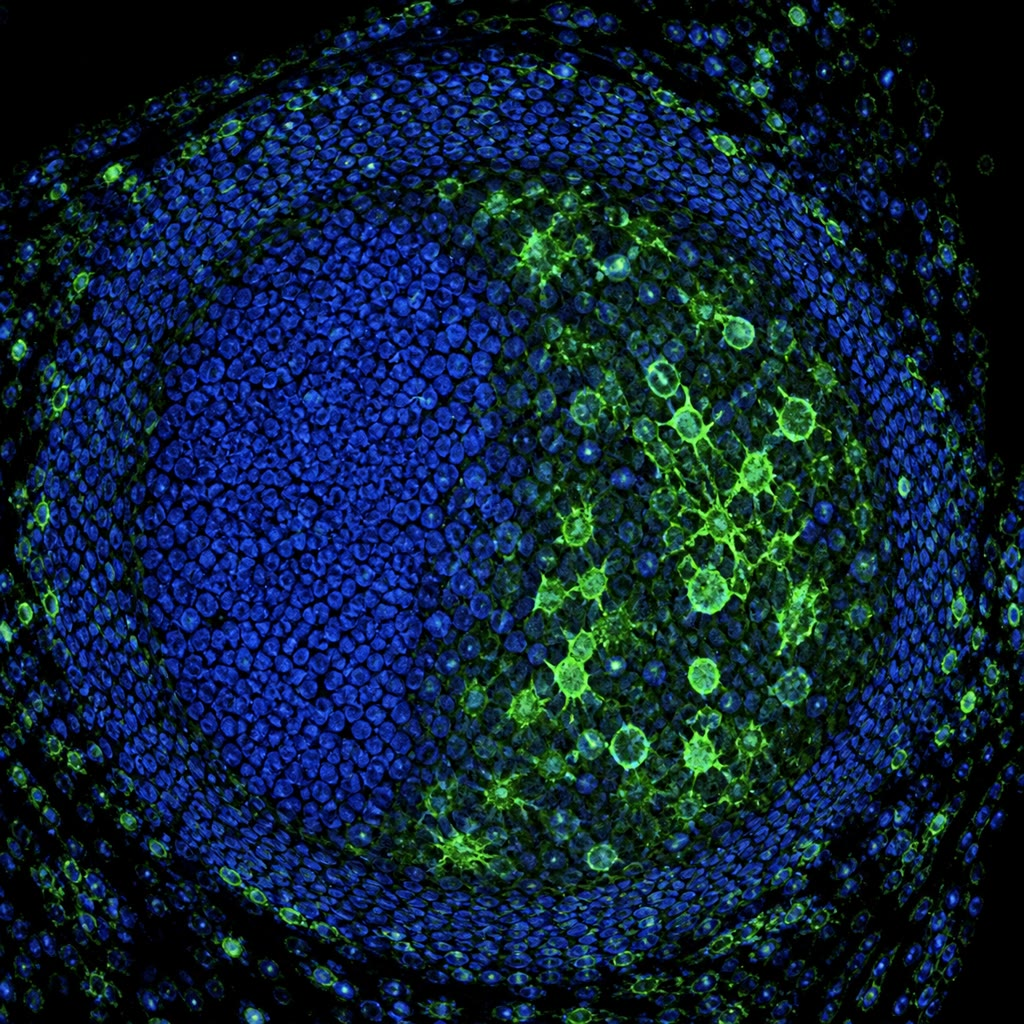
\includegraphics[width=0.36\linewidth]{images/book5/ai/b5-16-germinal-centre.jpg}\hspace{0.04\linewidth}
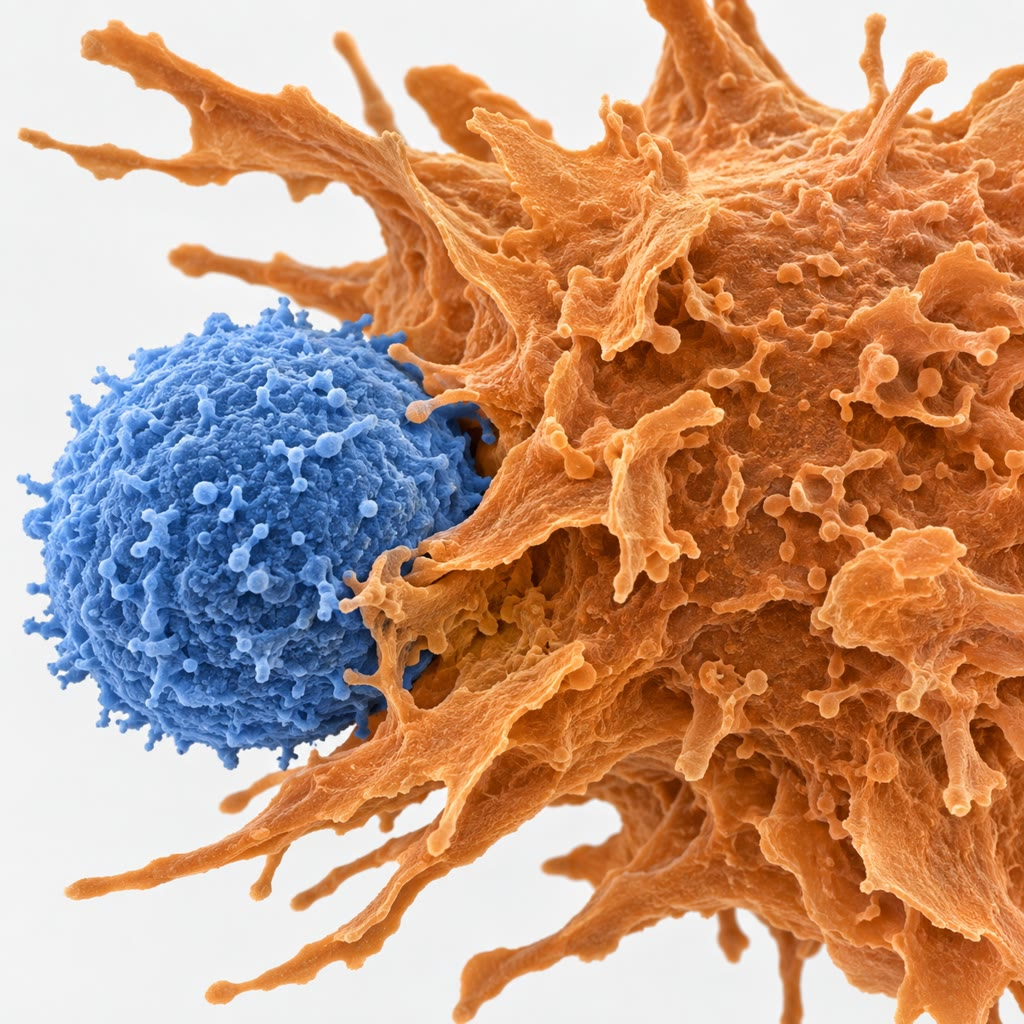
\includegraphics[width=0.36\linewidth]{images/book5/ai/b5-16-t-cell-apc.jpg}

{\small बाएँ: किसी \omterm{def:b3:adaptive-immunity:lymphocytes}{लसीका ग्रंथि} में कोई \omterm{def:b3:adaptive-immunity:germinal-centre}{जनन-केंद्र} --- भीड़ भरा गहरा
क्षेत्र और वरण का हलका क्षेत्र। दाएँ: किसी \omterm{def:b3:innate-immunity:innate}{वृक्षाभ कोशिका} के संपर्क में
कोई T~कोशिका (छोटी), यानी वह क्षण जिस पर अनुकूली अनुक्रिया तय होती है।}
\end{omfigure}

\section{सह्यता और उसकी विफलताएँ}

\begin{definition}[सह्यता]\label{def:b3:adaptive-immunity:tolerance}
\index{सह्यता}\index{ऋणात्मक वरण}\index{थाइमस}\index{ऐनर्जी}\index{FoxP3}\index{स्वप्रतिरक्षा}
संग्रह यादृच्छिक रूप से बनता है और इसलिए उसमें स्व के ग्राही भी होते
हैं। \emph{केंद्रीय सह्यता} उन्हें वहीं हटा देती है जहाँ वे कोशिकाएँ
परिपक्व होती हैं: थाइमस में वे T~कोशिकाएँ मार दी जाती हैं जिनके ग्राही
स्व पेप्टाइड--MHC को बहुत ज़ोर से बाँधें (\emph{ऋणात्मक वरण}), वे भी
मार दी जाती हैं जो MHC को बिलकुल नहीं बाँध पातीं (वे बेकार होतीं), और
केवल बीच के कुछ प्रतिशत ही निकलते हैं; कोई अनुलेखन कारक, AIRE, थाइमस की
कोशिकाओं से हर ऊतक के प्रोटीन अभिव्यक्त करवाता है --- इंसुलिन,
थायरोग्लोब्युलिन --- ताकि उनके लिए विशिष्ट T~कोशिकाएँ वहीं मिटाई जा
सकें। जो B~कोशिकाएँ मज्जा में स्व बाँधती हैं वे मिटा दी जाती हैं या
अपने ग्राही संपादित कर लेती हैं। \emph{परिधीय सह्यता} बाकी सँभालती है:
जो T~कोशिका अपने \omterm{def:b3:adaptive-immunity:lymphocytes}{प्रतिजन} से बिना \omterm{def:b3:adaptive-immunity:response}{सह-उद्दीपन} के मिले वह अनुक्रियाहीन कर
दी जाती है (\emph{ऐनर्जी}) या मिटा दी जाती है; और \emph{नियामक}
T~कोशिकाएँ, जिन्हें कारक FoxP3 परिभाषित करता है, स्व के विरुद्ध और
भोजन तथा सहभोजियों जैसे हानिरहित \omterm{def:b3:adaptive-immunity:lymphocytes}{प्रतिजनों} के विरुद्ध अनुक्रियाएँ
सक्रिय रूप से दबाती हैं। \emph{स्वप्रतिरक्षा} इन नियंत्रणों की विफलता
है: प्ररूप~1 मधुमेह (T~कोशिकाएँ $\beta$ कोशिकाएँ नष्ट करती हैं),
बहुखंडी काठिन्य (माइलिन), आमवाती संधिशोथ (संधियाँ), ल्यूपस (केंद्रकीय
घटकों के विरुद्ध \omterm{def:b3:adaptive-immunity:antibody}{प्रतिरक्षी}), अवटु रोग; हर एक कुछ ख़ास \omterm{def:b3:adaptive-immunity:mhc}{HLA}
युग्मविकल्पियों से जुड़ा है, जो संबंधित स्व पेप्टाइड प्रस्तुत करते हैं,
और कुछ ऐसे सूक्ष्मजीव के संक्रमण से छिड़ते हैं जिसके पेप्टाइड किसी स्व
प्रोटीन से मिलते-जुलते हैं (स्ट्रेप्टोकॉकी संक्रमण के बाद आमवाती ज्वर)।
\end{definition}

\begin{proof}[प्रमाण-सामग्री]
मेडावर (1953) ने एक अंतःप्रजनित चूहा-प्रभेद की कोशिकाएँ दूसरे प्रभेद
के नवजात चूहों में अंतःक्षिप्त कीं; वयस्क होने पर उन ग्रहीताओं ने दाता
प्रभेद की त्वचा-कलमें स्वीकार कर लीं, जिन्हें वे अन्यथा अस्वीकार कर
देते, जबकि तीसरे प्रभेदों की कलमें अस्वीकार करते रहे। \omterm{def:b3:adaptive-immunity:tolerance}{सह्यता} अर्जित
थी, विशिष्ट थी, और इससे तय होती थी कि प्रतिरक्षा-तंत्र जल्दी किससे
मिला --- यही बर्नेट के स्व-क्रियाशील क्लोनों के मिटाव का प्रायोगिक
आधार था। जो बच्चे प्रकार्यशील AIRE जीन के बिना जन्मते हैं उनमें एक साथ
कई अंगों के विरुद्ध \omterm{def:b3:adaptive-immunity:tolerance}{स्वप्रतिरक्षा} पनपती है; और जिनमें \omterm{def:b3:adaptive-immunity:tolerance}{FoxP3} न हो
(कोई दुर्लभ X-सहलग्न संलक्षण) उनमें शैशव में ही घातक \omterm{def:b3:adaptive-immunity:tolerance}{स्वप्रतिरक्षा} ---
यानी \omterm{def:b3:adaptive-immunity:tolerance}{सह्यता} की दोनों भुजाएँ, हर एक अपनी अनुपस्थिति से दिखाई गई।
\end{proof}

\begin{example}[अतिसंवेदनशीलता, न्यूनता, प्रत्यारोपण]\label{ex:b3:adaptive-immunity:failures}
\emph{एलर्जी} किसी हानिरहित \omterm{def:b3:adaptive-immunity:lymphocytes}{प्रतिजन} --- पराग, मूँगफली, पेनिसिलिन ---
के प्रति कोई Th2 अनुक्रिया है, जो IgE बनाती है; फिर से संसर्ग होने पर
वह \omterm{def:b3:adaptive-immunity:lymphocytes}{प्रतिजन} मास्ट कोशिकाओं पर बैठे IgE को आड़ा जोड़ देता है, जो मिनटों
में हिस्टामिन छोड़ देती हैं, और यदि वह \omterm{def:b3:adaptive-immunity:lymphocytes}{प्रतिजन} रक्त में हो तो यह
तंत्र-व्यापी मोचन \emph{तीव्रग्राहिता} है, जिसका उपचार एड्रिनैलीन से
होता है। \emph{प्रतिरक्षा-न्यूनता}: जिन बच्चों में \omterm{def:b3:adaptive-immunity:antibody}{RAG} या एंज़ाइम ADA न
हो वे कोई \omterm{def:b3:adaptive-immunity:lymphocytes}{लसीकाणु} नहीं बनाते (गंभीर संयुक्त प्रतिरक्षा-न्यूनता) और
मज्जा या जीन-चिकित्सा न मिले तो संक्रमण से मर जाते हैं; HIV CD4
T~कोशिकाएँ नष्ट कर देता है और उनके साथ वह मदद भी जो हर अनुक्रिया को
चाहिए। \emph{प्रत्यारोपण}: ग्रहीता की T~कोशिकाएँ दाता के \omterm{def:b3:adaptive-immunity:mhc}{HLA} अणुओं को
पराया देखती हैं, और सारी T~कोशिकाओं का दसवाँ भाग तक अनुक्रिया करता है
--- किसी भी रोगजनक के मुक़ाबले कहीं अधिक --- इसलिए कलमें \omterm{def:b3:adaptive-immunity:mhc}{HLA} स्थलों पर
मिलाई जाती हैं और ग्रहीता जीवन भर प्रतिरक्षा-दमित रखा जाता है; मज्जा
की कोई कलम उलटे अपने नए परपोषी पर ही वार कर सकती है। और जान-बूझकर किए
गए उपयोग: \cref{ch:b3:genetic-engineering} के \omterm{def:b3:genetic-engineering:expression}{एकक्लोनी प्रतिरक्षी}, वे
\omterm{prop:b3:cancer-biology:immune}{जाँच-बिंदु निरोधक} जो T~कोशिकाओं को \omterm{def:b3:cancer-biology:hallmarks}{अर्बुदों} पर छोड़ देते हैं
(\cref{ch:b3:cancer-biology}), और किसी अर्बुद-प्रतिजन के लिए काइमेरी
ग्राही से अभियंत्रित T~कोशिकाएँ (CAR-T), जिन्होंने वे रक्तकर्कट ठीक
किए हैं जिन्हें और कुछ छू भी नहीं पाता था।
\end{example}

\section{टीकाकरण}

\begin{definition}[टीके और सामूहिक प्रतिरक्षा]\label{def:b3:adaptive-immunity:vaccine}
\index{टीका}\index{सामूहिक प्रतिरक्षा}\index{मूल जनन संख्या}\index{टीका-सामर्थ्य}
कोई \emph{टीका} किसी रोगजनक के \omterm{def:b3:adaptive-immunity:lymphocytes}{प्रतिजन} किसी सहवर्धक के साथ, या किसी
ऐसे रूप में जो जन्मजात ग्राही छेड़ दे, प्रस्तुत करता है, ताकि ग्रहीता
बिना रोग के ही \omterm{def:b3:adaptive-immunity:response}{स्मृति कोशिकाएँ} और \omterm{def:b3:adaptive-immunity:antibody}{प्रतिरक्षी} पा ले
(\cref{ch:b3:virology} उसके प्रकार गिनाता है)। उसका \emph{सामर्थ्य}
$E$ टीकाकृत लोगों का वह अंश है जो सुरक्षित होता है। सुरक्षा टीकाकृतों से
आगे भी जाती है: कोई रोगजनक जो किसी ऐसी समष्टि में फैले जहाँ सब संवेद्य
होने पर हर मामला औसतन $R_{0}$ दूसरों को संक्रमित करता हो --- यानी
\emph{मूल जनन संख्या} --- वह कुछ लोगों के प्रतिरक्षित होने पर केवल
संवेद्य अंश के $R_{0}$ गुने को संक्रमित करता है, और जब वह संख्या एक से
नीचे गिरे तब मिट जाता है। यही \emph{सामूहिक प्रतिरक्षा} है: प्रतिरक्षित
लोगों की किसी देहली के ऊपर संचरण की शृंखला टूट जाती है और अटीकाकृत ---
शिशु, प्रतिरक्षा-दुर्बल, वे जिनमें टीका विफल रहा --- बाकियों से
सुरक्षित हो जाते हैं।
\end{definition}

\begin{theorem}[सामूहिक प्रतिरक्षा की देहली]\label{thm:b3:adaptive-immunity:herd}
\index{सामूहिक प्रतिरक्षा!देहली}\index{SIR प्रतिरूप}
किसी ऐसी समष्टि में जिसका अंश $p$ प्रतिरक्षित हो और बाकी संवेद्य, हर
मामला औसतन $R_{\text{प्रभावक}} = R_{0}(1 -
p)$ दूसरों को संक्रमित करता है। कोई महामारी शुरू ही नहीं हो सकती यदि
$R_{\text{प्रभावक}} < 1$ हो, यानी यदि
\[
p > p_{c} = 1 - \frac{1}{R_{0}} .
\]
सामर्थ्य $E$ वाले किसी टीके के साथ ज़रूरी आच्छादन $f_{c} = p_{c}/E$ है।
यदि कोई महामारी किसी संवेद्य समष्टि में चल ही पड़े (\omterm{thm:b3:adaptive-immunity:herd}{SIR प्रतिरूप},
संक्रमण-दर $\beta$ और स्वास्थ्यलाभ-दर $\gamma$ के साथ, $R_{0} =
\beta/\gamma$), तो वह तब शिखर छूती है जब संवेद्य अंश गिरकर
$1/R_{0}$ रह जाए, और वह अंश जो कभी संक्रमित नहीं हुआ, $s_{\infty}$,
$\ln s_{\infty} = -R_{0}(1 - s_{\infty})$ को संतुष्ट करता है।
\end{theorem}
\begin{proof}
हर मामला ऐसे संपर्क बनाता है जो सबके संवेद्य होने पर $R_{0}$ लोगों को
संक्रमित करते; उनका अंश $1 - p$ ही संवेद्य है, इसलिए $R_{\text{प्रभावक}} =
R_{0}(1-p)$, और शर्त $R_{\text{प्रभावक}} < 1$ से $p_{c}$ मिलता है; जो \omterm{def:b3:adaptive-immunity:vaccine}{टीका}
पाने वालों के अंश $E$ की रक्षा करे वह समष्टि का अंश $Ef$ प्रतिरक्षित
बना देता है, इसलिए $Ef > p_{c}$। \omterm{thm:b3:adaptive-immunity:herd}{SIR प्रतिरूप} में,
$\mathrm{d}s/\mathrm{d}t = -\beta si$ और $\mathrm{d}i/\mathrm{d}t =
\beta si - \gamma i = \gamma i(R_{0}s - 1)$, इसलिए $i$ तब तक बढ़ता है जब तक $s >
1/R_{0}$ हो और उसके बाद घटता है: शिखर $s = 1/R_{0}$ पर है। दोनों
समीकरणों को भाग देने पर $\mathrm{d}i/\mathrm{d}s = -1 + 1/(R_{0}s)$,
इसलिए $i + s -
\ln s/R_{0}$ अचर है; उसे आरंभ पर ($s = 1$, $i
\approx 0$) और अंत पर ($i = 0$, $s = s_{\infty}$) आँकने पर
$s_{\infty} - \ln s_{\infty}/R_{0} = 1$ मिलता है, यानी अंतिम-आकार संबंध।
\end{proof}

\begin{example}[खसरा और चेचक]\label{ex:b3:adaptive-immunity:measles}
खसरे का $R_{0} \approx 15$ है: $p_{c} = 1 - 1/15 = 93\,\%$, और दो
मात्राओं के बाद $97\,\%$ सामर्थ्य वाले किसी टीके के साथ ज़रूरी आच्छादन
$96\,\%$ है --- इसीलिए जहाँ कहीं टीकाकरण कुछ प्रतिशत फिसलता है वहाँ
खसरा लौट आता है, और इसीलिए अच्छे टीकाकरण वाले किसी देश में कोई अटीकाकृत
बच्चा फिर भी सुरक्षित है। चेचक का $R_{0} \approx 5$--$7$ था, देहली
$80$--$85\,\%$ के पास, कोई पशु-भंडार नहीं, कोई अलक्षणी वाहक नहीं, और
एक ही मात्रा में काम करता \omterm{def:b3:adaptive-immunity:vaccine}{टीका}: उन्मूलन-योग्य, और उन्मूलित। पोलियो
लगभग वहीं पहुँच चुका है। इन्फ़्लुएंज़ा और कोरोना \omterm{def:b3:virology:virus}{विषाणु}, जिनके \omterm{def:b3:adaptive-immunity:lymphocytes}{प्रतिजन}
अपवाहित होते हैं (\cref{ch:b3:virology}) और जिनकी प्रतिरक्षा घटती है,
नहीं हैं। किसी अटीकाकृत समष्टि में $R_{0} = 3$ वाली कोई महामारी,
अंतिम-आकार संबंध से, लोगों के $1 - s_{\infty} = 94\,\%$ को संक्रमित
करती है; $R_{0} = 1.5$ के साथ $58\,\%$ को।
\end{example}

\begin{omfigure}
\begin{tikzpicture}
\begin{axis}[
  width=6.4cm, height=5.4cm,
  axis x line=bottom, axis y line=left,
  xmin=1, xmax=18, ymin=0, ymax=1,
  xlabel={$R_{0}$}, ylabel={देहली $p_{c}$},
  xlabel style={font=\small, at={(axis description cs:0.5,-0.12)}, anchor=north}, ylabel style={font=\small},
  tick label style={font=\scriptsize}, xtick={1,3,6,9,12,15,18}, ytick={0,0.5,0.8,0.93,1}, yticklabels={0,0.5,0.8,0.93,1},
  clip=false,
]
\addplot[very thick, omDef, domain=1:18, samples=80] {1-1/x};
\fill[omThm] (axis cs:15,0.933) circle (2pt); \node[font=\scriptsize, anchor=south east] at (axis cs:15,0.94) {खसरा};
\fill[omThm] (axis cs:6,0.833) circle (2pt); \node[font=\scriptsize, anchor=north west] at (axis cs:6.3,0.82) {चेचक};
\fill[omThm] (axis cs:2.5,0.6) circle (2pt); \node[font=\scriptsize, anchor=north west] at (axis cs:2.6,0.58) {1918 का इन्फ़्लुएंज़ा};
\end{axis}
\begin{axis}[
  at={(7.6cm,0)}, anchor=south west,
  width=6.4cm, height=5.4cm,
  axis x line=bottom, axis y line=left,
  xmin=0, xmax=60, ymin=0, ymax=0.35,
  xlabel={दिन}, ylabel={संक्रामक अंश},
  xlabel style={font=\small, at={(axis description cs:0.5,-0.12)}, anchor=north}, ylabel style={font=\small},
  tick label style={font=\scriptsize}, xtick={0,20,40,60}, ytick={0,0.1,0.2,0.3},
  clip=false,
]
\addplot[very thick, omThm, smooth] coordinates {(0,0.001) (5,0.003) (10,0.012) (15,0.04) (20,0.12) (25,0.25) (28,0.30) (31,0.27) (35,0.18) (40,0.09) (45,0.04) (50,0.015) (55,0.006) (60,0.002)};
\addplot[very thick, omDef, smooth] coordinates {(0,0.001) (5,0.0015) (10,0.0025) (15,0.004) (20,0.006) (25,0.009) (30,0.012) (35,0.014) (40,0.015) (45,0.014) (50,0.012) (55,0.009) (60,0.007)};
\node[font=\scriptsize, omThm, anchor=west] at (axis cs:30,0.3) {कोई प्रतिरक्षा नहीं, $R_{0} = 3$};
\node[font=\scriptsize, omDef, anchor=south west] at (axis cs:32,0.03) {\qty{60}{\%} टीकाकृत: $R_{\text{प्रभावक}} = 1.2$};
\end{axis}
\end{tikzpicture}

{\small बाएँ: देहली $1 - 1/R_{0}$ --- रोग जितना अधिक संक्रामक, उतना ही
सबके निकट तक प्रतिरक्षित होना पड़ता है। दाएँ: किसी अनुभवहीन समष्टि में
और \qty{60}{\%} प्रतिरक्षित समष्टि में $R_{0} = 3$ वाली कोई SIR
महामारी, जो उसे रोकने के लिए तो पर्याप्त नहीं पर उसे चपटा और धीमा कर
देती है।}
\end{omfigure}

\begin{omfigure}
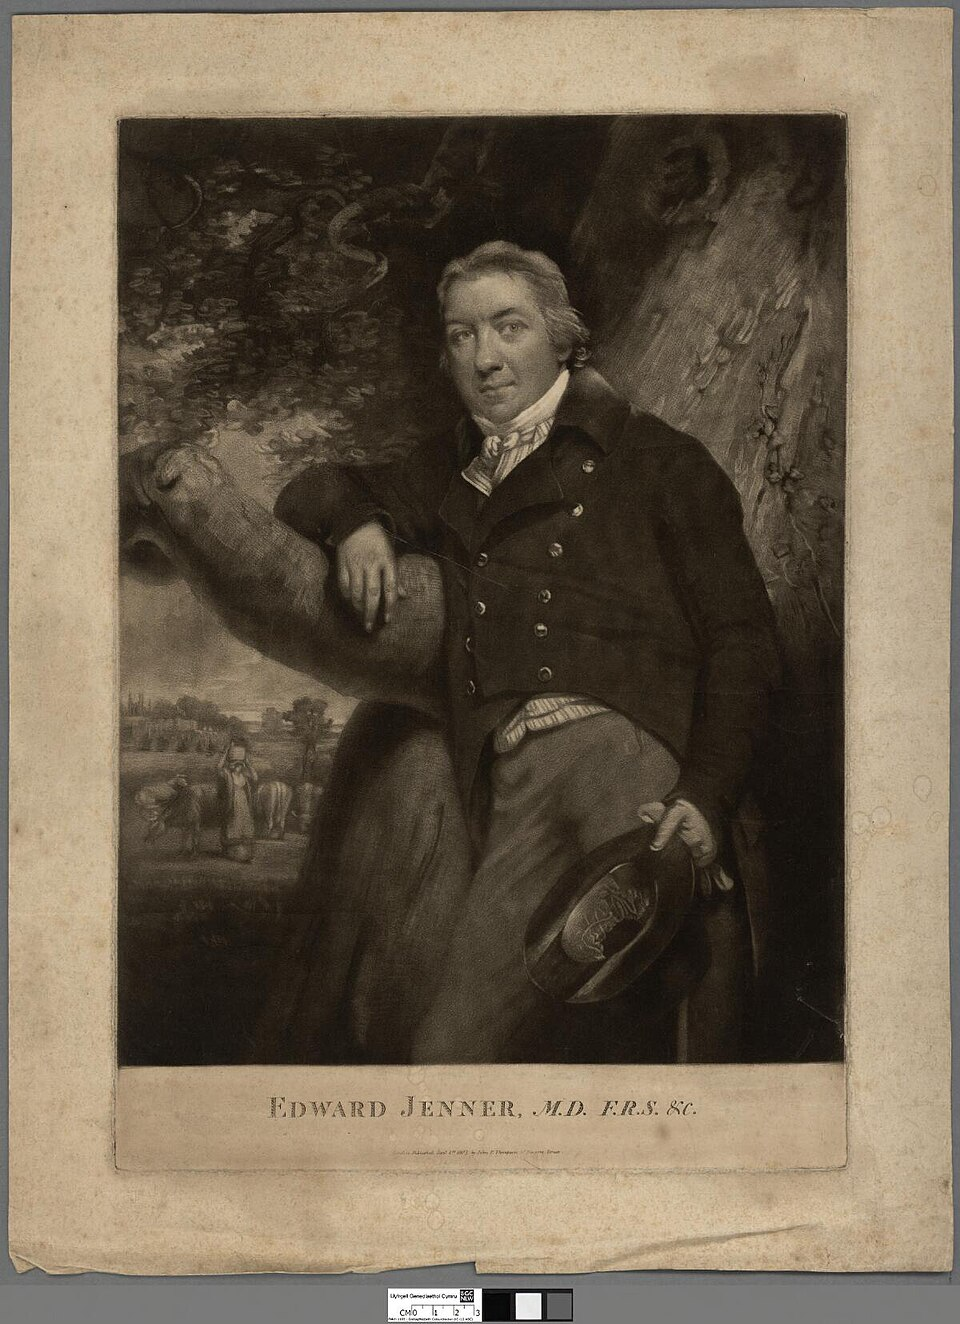
\includegraphics[width=0.30\linewidth]{images/book5/jenner.jpg}\hspace{0.04\linewidth}
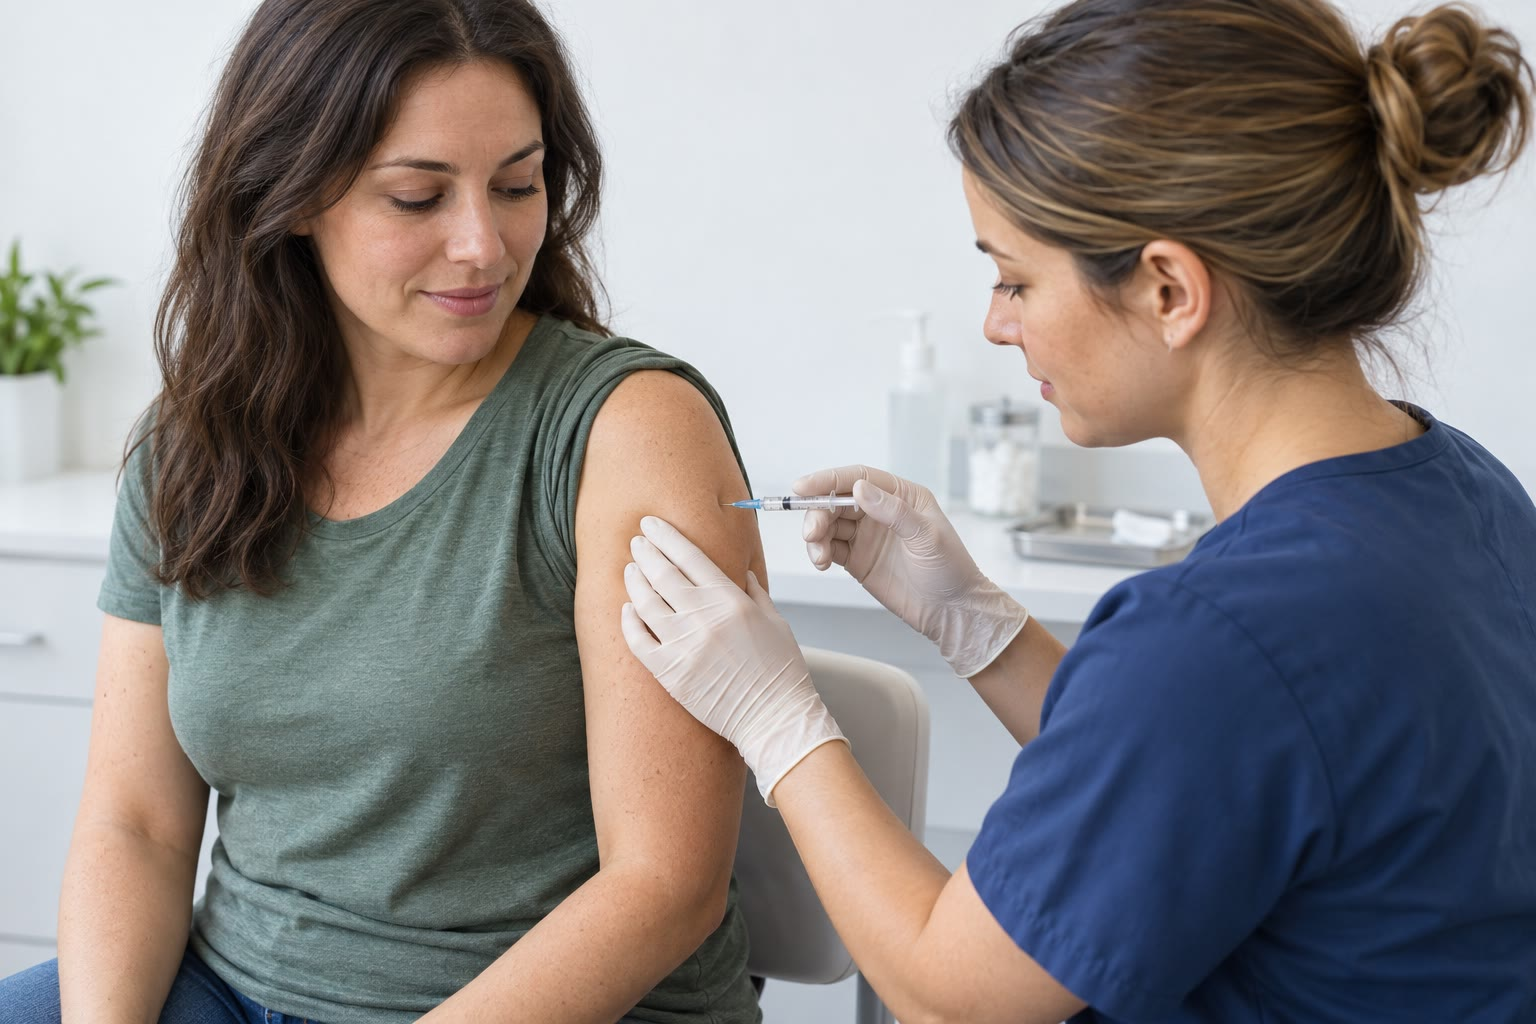
\includegraphics[width=0.50\linewidth]{images/book5/ai/b5-16-vaccination.jpg}

{\small एडवर्ड जेनर, जिसने 1796 में किसी लड़के को गोशीतला से चेचक के
विरुद्ध बचाया और टीकाकरण की नींव रखी (1807 का उत्कीर्णन, सार्वजनिक)।
दाएँ: दो सदियों बाद वही काम --- कोई अंतःपेशीय \omterm{def:b3:adaptive-immunity:vaccine}{टीका}, जिसका \omterm{def:b3:adaptive-immunity:lymphocytes}{प्रतिजन}
अंसच्छद की \omterm{def:b3:innate-immunity:innate}{वृक्षाभ कोशिकाएँ} कक्षीय \omterm{def:b3:adaptive-immunity:lymphocytes}{लसीका ग्रंथियों} तक ले जाएँगी।}
\end{omfigure}

\begin{remark}[प्रतिरक्षा क्या याद रखती है]\label{rem:b3:adaptive-immunity:memory}
अनुकूली प्रतिरक्षा-तंत्र हममें से हर एक के भीतर बैठा कोई डार्विनी यंत्र
है: यादृच्छिक विचरण (V(D)J, अतिउत्परिवर्तन), वरण (\omterm{def:b3:adaptive-immunity:lymphocytes}{प्रतिजन} द्वारा,
\omterm{def:b3:adaptive-immunity:germinal-centre}{जनन-केंद्र} में, \omterm{def:b3:adaptive-immunity:tolerance}{थाइमस} में स्व के विरुद्ध) और वंशागति (\omterm{def:b3:adaptive-immunity:response}{स्मृति कोशिकाएँ},
क्लोनी विस्तार)। वह हफ़्तों में वह समस्या हल कर देता है जिसे विकास
सहस्राब्दियों में हल करता है --- कोई ऐसा अणु जो पहले कभी न देखे गए
किसी लक्ष्य को बाँधे --- और उसके उत्तर सीधे देखे गए विकास के सबसे
अच्छी तरह अध्ययन किए गए उदाहरणों में हैं। उसकी कीमत \omterm{def:b3:adaptive-immunity:tolerance}{स्वप्रतिरक्षा} है,
जन्मजात तंत्र के निर्णय पर उसकी निर्भरता पूर्ण है, और उसकी स्मृति,
जिसका दोहन जेनर ने किया और जिसे टीके जान-बूझकर लिखते हैं, वही कारण है
कि दीर्घजीवी, धीमे जनने वाले प्राणियों की कोई जाति तेज़ जनने वाले
सूक्ष्मजीवों की दुनिया में टिक सकती है।
\end{remark}

\section{अभ्यास}

\begin{exercise}[$\star$]\label{exo:b3:adaptive-immunity:1}
\omterm{def:b3:adaptive-immunity:lymphocytes}{क्लोनी वरण} के चारों सिद्धांत बताइए, और पहले दो में से हर एक का समर्थन
करता प्रयोग।
\end{exercise}

\begin{exercise}[$\star$]\label{exo:b3:adaptive-immunity:2}
किसी \omterm{def:b3:adaptive-immunity:antibody}{प्रतिरक्षी} की संरचना का वर्णन कीजिए और पाँचों वर्गों में से हर एक
का प्रकार्य बताइए।
\end{exercise}

\begin{exercise}[$\star$]\label{exo:b3:adaptive-immunity:3}
\omterm{def:b3:adaptive-immunity:mhc}{MHC वर्ग~I} और वर्ग~II की तुलना कीजिए: कोशिका-वितरण, पेप्टाइड का स्रोत,
पेप्टाइड की लंबाई, और हर एक को पढ़ती T~कोशिका।
\end{exercise}

\begin{exercise}[$\star$]\label{exo:b3:adaptive-immunity:4}
$R_{0}$ और \omterm{def:b3:adaptive-immunity:vaccine}{सामूहिक प्रतिरक्षा} की देहली परिभाषित कीजिए, और गलसुआ
($R_{0} = 5$), कुकर खाँसी ($R_{0} = 12$) तथा 1918 के इन्फ़्लुएंज़ा
($R_{0} = 2.5$) के लिए देहली निकालिए।
\end{exercise}

\begin{exercise}[$\star\star$]\label{exo:b3:adaptive-immunity:5}
किसी जाति के $V_{H} = 50$, $D = 20$, $J_{H} = 5$ हैं और उसका एक ही
हल्का स्थल है जिसमें $V = 60$, $J = 4$। संचयात्मक संग्रह निकालिए, फिर
$10^{4}$ के संधि-गुणक के साथ कुल। उस प्राणी की $10^{9}$ B~कोशिकाओं से
वह कैसा बैठता है?
\end{exercise}

\begin{exercise}[$\star\star$]\label{exo:b3:adaptive-immunity:6}
किसी \omterm{def:b3:adaptive-immunity:germinal-centre}{जनन-केंद्र} की B~कोशिका का परिवर्ती क्षेत्र \qty{1000}{bp} है; AID
प्रति विभाजन प्रति क्षार-युग्म $10^{-3}$ की दर से उत्परिवर्तित करती
है। $20$ विभाजनों में प्रति कोशिका कितने उत्परिवर्तन, और $10^{5}$
कोशिकाओं के बीच उस \omterm{def:b3:adaptive-immunity:antibody}{प्रतिरक्षी} के कितने भिन्न एक-क्षार प्रभेद बनते हैं?
$3000$ संभव एकल प्रतिस्थापनों से तुलना कीजिए।
\end{exercise}

\begin{exercise}[$\star\star$]\label{exo:b3:adaptive-immunity:7}
समझाइए कि किसी एक व्यक्ति की T~कोशिका दूसरे व्यक्ति की कोशिकाओं द्वारा
प्रस्तुत विषाणुजन्य पेप्टाइड क्यों नहीं पहचानती, और यही तथ्य
प्रत्यारोपण को कठिन तथा \omterm{def:b3:adaptive-immunity:mhc}{HLA} तंत्र को बहुरूपी क्यों बनाता है।
\end{exercise}

\begin{exercise}[$\star\star$]\label{exo:b3:adaptive-immunity:8}
उस बच्चे के प्रतिरक्षा-लक्षणरूप का पूर्वानुमान कीजिए जिसमें (क) RAG1,
(ख) AIRE, (ग) \omterm{def:b3:adaptive-immunity:tolerance}{FoxP3}, (घ) \omterm{def:b3:adaptive-immunity:antibody}{वर्ग-परिवर्तन} एंज़ाइम AID, और (ङ) CD4 T~कोशिकाएँ न हों।
\end{exercise}

\begin{exercise}[$\star\star$]\label{exo:b3:adaptive-immunity:9}
किसी टीके का सामर्थ्य \qty{90}{\%} है और उस रोग का $R_{0} = 6$। कौन-सा
आच्छादन संचरण रोक देता है? यदि आच्छादन \qty{80}{\%} हो तो
$R_{\text{प्रभावक}}$ क्या है, और कोई महामारी समष्टि के किस अंश को संक्रमित
करती है (अंतिम-आकार संबंध में $R_{0}$ की जगह संवेद्यों के बीच
$R_{\text{प्रभावक}}$ रखिए --- या तर्क दीजिए कि वह लगभग क्यों ठीक है)?
\end{exercise}

\begin{exercise}[$\star\star\star$]\label{exo:b3:adaptive-immunity:10}
प्रमेय का अंतिम-आकार संबंध SIR समीकरणों से व्युत्पन्न कीजिए और उसे
$R_{0} = 1.5$, $2$, $3$ तथा $5$ के लिए संख्यात्मक रूप से हल कीजिए। कोई
महामारी बिना किसी हस्तक्षेप के भी सबको संक्रमित क्यों नहीं करती?
\end{exercise}

\begin{exercise}[$\star\star\star$]\label{exo:b3:adaptive-immunity:11}
\omterm{def:b3:adaptive-immunity:germinal-centre}{बंधुता-परिपक्वन} तीन सप्ताह में बंधन हज़ार गुना बढ़ा देता है। \omterm{def:b3:adaptive-immunity:germinal-centre}{जनन-केंद्र}
को वरण के अंतर्गत किसी समष्टि की तरह लीजिए: प्रति कोशिका प्रति विभाजन
एक उत्परिवर्तन की दर के साथ, जिनमें से अंश $10^{-2}$ बंधुता को गुणक
$1.5$ से सुधारता हो और बाकी उदासीन या हानिकारक हों, हज़ार गुनी बढ़त के
लिए वरण के कितने चक्र चाहिए, और हर चक्र को कितनी कोशिकाएँ छाननी
पड़ेंगी? टिप्पणी कीजिए कि \omterm{def:b3:adaptive-immunity:germinal-centre}{जनन-केंद्र} चक्रों में क्यों संगठित है।
\end{exercise}

\begin{exercise}[$\star\star\star$]\label{exo:b3:adaptive-immunity:12}
स्वप्रतिरक्षी रोग स्त्रियों में अधिक आम हैं और \omterm{def:b3:adaptive-immunity:mhc}{HLA} युग्मविकल्पियों से
जुड़े हैं; धनी देशों में प्ररूप~1 मधुमेह पचास वर्षों में पाँच गुना बढ़ा
है। इस अध्याय के और \cref{ch:b3:microbiomes} के तंत्रों से हर प्रेक्षण
की व्याख्याएँ सुझाइए और हर एक की एक-एक जाँच।
\end{exercise}

\section{समस्या: कोई टीका-अभियान}

\begin{problem}[{सप्तांत समस्या --- कोई संग्रह गिना गया, कोई अनुक्रिया
सौ कोशिकाओं से एक मिलीलीटर सीरम तक समयबद्ध की गई, कोई जनन-केंद्र किसी
विकासीय कलन-विधि की तरह चलाया गया, और खसरे का कोई अभियान सामूहिक देहली
के सामने नियोजित किया गया, जिसका अंत संग्रह के आकार पर होता है, उस
प्रतिरक्षी पर जो कोई प्लाज़्मा कोशिका दिन भर में बनाती है, और उस
आच्छादन पर जो किसी देश को चाहिए}]
\label{pb:b3:adaptive-immunity:1}
आँकड़े: $V_{H} = 40$, $D = 25$, $J_{H} = 6$; हल्के स्थल $(40, 5)$ और
$(30, 4)$; संधि-गुणक $3\times 10^{4}$। किसी शरीर में $10^{11}$
B~कोशिकाएँ हैं; $10^{5}$ में एक कोई दिया एपिटोप बाँधती है; $100$
पूर्वज भर्ती किए जाते हैं; $7$ दिनों तक हर \qty{8}{h} में विभाजन;
क्लोन का \qty{30}{\%} \omterm{def:b3:adaptive-immunity:response}{प्लाज़्मा कोशिकाएँ} बन जाता है, जिनमें से हर एक
प्रति सेकंड $2000$ IgG अणु स्रवित करती है; IgG \qty{150}{kDa} का है;
प्लाज़्मा-आयतन \qty{3}{L}; IgG का अर्ध-आयु काल \qty{21}{d}।
\omterm{def:b3:adaptive-immunity:germinal-centre}{जनन-केंद्र}: \qty{1000}{bp} का परिवर्ती क्षेत्र, प्रति bp प्रति विभाजन
$10^{-3}$ उत्परिवर्तन, $100$ में एक उत्परिवर्तन बंधुता $1.5$ गुना
सुधारता है। खसरा: $R_{0} = 15$, \omterm{def:b3:adaptive-immunity:vaccine}{टीका-सामर्थ्य} एक मात्रा के बाद $0.93$
और दो के बाद $0.97$; $5\times 10^{6}$ लोगों का कोई देश जिसमें साल में
$60\,000$ जन्म होते हैं।

\medskip
\noindent\textbf{भाग I --- संग्रह।}
\begin{enumerate}
  \item संचयात्मक संग्रह और \omterm{def:b3:adaptive-immunity:antibody}{संधि-विविधता} के साथ कुल निकालिए।
  \item B~कोशिकाओं की संख्या से तुलना कीजिए। कोई एक शरीर किसी एक समय
        संभव संग्रह का कितना अंश अभिव्यक्त करता है, और दो व्यष्टियों के
        संग्रहों के लिए इससे क्या निकलता है?
  \item शरीर में कितनी B~कोशिकाएँ उस एपिटोप को बाँधती हैं? $10^{8}$
        B~कोशिकाएँ रखती किसी \omterm{def:b3:adaptive-immunity:lymphocytes}{लसीका ग्रंथि} में औसतन कितनी?
  \item किसी नवजात में $10^{9}$ B~कोशिकाएँ हैं। कितनी उस एपिटोप को
        बाँधती हैं, और फिर भी नवजात की अनुक्रिया कमज़ोर क्यों है?
  \item किसी \omterm{def:b3:adaptive-immunity:antibody}{प्रतिरक्षी} का तीसरा भारी-शृंखला पाश \omterm{def:b3:adaptive-immunity:antibody}{संधि-विविधता} से बनता
        है। समझाइए कि यह पाश उस अणु का सबसे परिवर्ती भाग क्यों है और
        प्रायः बंधक स्थल के केंद्र में क्यों।
  \item \omterm{def:b3:adaptive-immunity:germinal-centre}{कायिक अतिउत्परिवर्तन} वरण के बाद विविधता जोड़ता है, V(D)J पहले।
        दोनों का, उसी क्रम में, होना लाभदायक क्यों है?
\end{enumerate}

\medskip
\noindent\textbf{भाग II --- अनुक्रिया।}
\begin{enumerate}[resume]
  \item हर \qty{8}{h} में बँटती $100$ कोशिकाओं से $7$ दिनों बाद कितनी?
        कितनी \omterm{def:b3:adaptive-immunity:response}{प्लाज़्मा कोशिकाएँ}?
  \item वे प्रति दिन कितने IgG अणु स्रवित करती हैं, और कितना
        द्रव्यमान? एक दिन की उपज \qty{3}{L} में कौन-सी सीरम-सांद्रता
        देती है?
  \item क्षय छोड़कर, उसी दर से दस दिन स्रवण के बाद सांद्रता g/L में
        क्या है? \qty{10}{g/L} के सामान्य कुल IgG से तुलना कीजिए।
  \item \omterm{def:b3:adaptive-immunity:response}{प्लाज़्मा कोशिकाएँ} दो सप्ताह बाद मर जाती हैं; फिर वह \omterm{def:b3:adaptive-immunity:antibody}{प्रतिरक्षी}
        \qty{21}{d} के अर्ध-आयु काल से क्षीण होता है। प्रश्न 9 की
        सांद्रता को सौ गुना गिरने में कितना समय लगता है? वर्षों तक
        \omterm{def:b3:adaptive-immunity:antibody}{प्रतिरक्षी} कौन बनाए रखता है?
  \item कोई द्वितीयक अनुक्रिया $10^{5}$ \omterm{def:b3:adaptive-immunity:response}{स्मृति कोशिकाओं} से शुरू होती
        है। $3$ दिनों बाद कितनी कोशिकाएँ, और वह प्राथमिक अनुक्रिया के
        दिन 3 तथा दिन 7 से कैसी बैठती है?
  \item समझाइए कि किसी प्राथमिक अनुक्रिया में IgM पहले और IgG बाद में
        क्यों आता है, और द्वितीयक अनुक्रिया शुरू से ही IgG क्यों होती है।
\end{enumerate}

\medskip
\noindent\textbf{भाग III --- \omterm{def:b3:adaptive-immunity:germinal-centre}{जनन-केंद्र}।}
\begin{enumerate}[resume]
  \item कोई B~कोशिका अपने परिवर्ती क्षेत्र में प्रति विभाजन कितने
        उत्परिवर्तन पाती है? $20$ विभाजनों में?
  \item किसी एक विभाजन की संततियों का कितना अंश कोई सुधारक उत्परिवर्तन
        ढोता है? $10^{4}$ बँटती कोशिकाओं वाले किसी \omterm{def:b3:adaptive-immunity:germinal-centre}{जनन-केंद्र} में
        प्रति विभाजन कितनी सुधरी कोशिकाएँ प्रकट होती हैं?
  \item $1.5$ के कितने क्रमिक सुधार बंधुता में हज़ार गुनी बढ़त देते
        हैं? यदि वरण के हर चक्र में दो विभाजन लगें (\qty{12}{h}), तो
        वह कितना समय हुआ?
  \item अधिकांश उत्परिवर्तन \omterm{def:b3:adaptive-immunity:antibody}{प्रतिरक्षी} को नुक़सान पहुँचाते हैं। यदि
        \qty{50}{\%} उत्परिवर्तन बंधन नष्ट कर दें, तो हर विभाजन के
        उत्परिवर्तन से कोशिकाओं का कितना अंश बचता है, और हलके क्षेत्र
        को अधिकांश कोशिकाएँ क्यों मारनी पड़ती हैं?
  \item छह सप्ताह के अंतर पर दो मात्राओं में दिया गया कोई \omterm{def:b3:adaptive-immunity:vaccine}{टीका} एक
        मात्रा से ऊँची बंधुता के \omterm{def:b3:adaptive-immunity:antibody}{प्रतिरक्षी} देता है। \omterm{def:b3:adaptive-immunity:germinal-centre}{जनन-केंद्र} से
        समझाइए।
  \item कुछ \omterm{def:b3:virology:virus}{विषाणु} (HIV, इन्फ़्लुएंज़ा) अपना पृष्ठ उत्परिवर्तित करके
        \omterm{def:b3:adaptive-immunity:antibody}{प्रतिरक्षियों} से बच निकलते हैं। समझाइए कि फिर भी \omterm{def:b3:adaptive-immunity:germinal-centre}{जनन-केंद्र} ही
        किसी व्यापक रूप से रक्षक टीके की आशा का आधार क्यों है।
\end{enumerate}

\medskip
\noindent\textbf{भाग IV --- अभियान।}
\begin{enumerate}[resume]
  \item खसरे के लिए सामूहिक देहली, और एक मात्रा के साथ ज़रूरी आच्छादन;
        दो मात्राओं के साथ।
  \item वह देश \qty{90}{\%} बच्चों को दो मात्राएँ लगाता है। प्रतिरक्षित
        अंश, $R_{\text{प्रभावक}}$, और निर्णय: क्या खसरा फैलता रहता है?
  \item \qty{90}{\%} आच्छादन पर जन्मों के हर वर्ष कितने संवेद्य बच्चे
        जमा होते हैं (अटीकाकृत जमा टीका-विफलताएँ)? खसरे के बिना पाँच
        वर्षों के बाद कितने संवेद्य होते हैं, और तब कोई आयात क्यों
        प्रकोप ले आता है?
  \item संवेद्यों के बीच प्रभावी जनन संख्या के साथ अंतिम-आकार संबंध का
        उपयोग करके आँकिए कि कोई प्रकोप उन संवेद्यों के किस अंश को
        संक्रमित करता है। (प्रश्न 20 का $R_{\text{प्रभावक}}$ पूरी समष्टि
        की जनन संख्या के रूप में लीजिए, और ध्यान दीजिए कि संवेद्य समूह
        के भीतर वह रोग ऐसे फैलता है मानो $R_{0}$ ही $R_{\text{प्रभावक}}$
        हो।)
  \item आच्छादन दो मात्राओं के साथ \qty{95}{\%} तक उठाया जाता है।
        प्रतिरक्षित अंश और $R_{\text{प्रभावक}}$; क्या देहली पूरी होती है?
  \item एक वर्ष से छोटे शिशुओं को खसरे का \omterm{def:b3:adaptive-immunity:vaccine}{टीका} नहीं लगाया जा सकता और
        उन्हीं के उससे मरने की सबसे अधिक संभावना है। समझाइए कि वह
        अभियान उनकी रक्षा कैसे करता है, और आच्छादन \qty{85}{\%} तक गिर
        जाए तो उनकी सुरक्षा का क्या होता है।
  \item सारांश दीजिए: कुल संग्रह (प्रश्न~1), एक दिन की \omterm{def:b3:adaptive-immunity:response}{प्लाज़्मा
        कोशिकाएँ} जितना IgG बनाती हैं (प्रश्न~8), और देश को चाहिए
        दो-मात्रा आच्छादन (प्रश्न~19)।
\end{enumerate}
\end{problem}
